\chapter*{Avant-propos}

\section*{\og Technologies informatiques \fg{}}

\begin{minipage}[H]{0.3\linewidth}
  \begin{figure}[H]
  \centering
  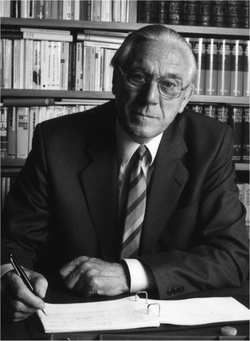
\includegraphics[width=0.8\textwidth]{../resources/illustrations/steinbuch}
  \caption{Karl Steinbuch}
  \end{figure}
\end{minipage}
\begin{minipage}[H]{0.7\linewidth}
Le mot \textbf{informatique} est une concaténation d'\textbf{information} et d'\textbf{automatique} faite en 1957 par Karl Steinbuch\cite{steinbuch-2005} pour décrire le traitement automatique de l'information.

Depuis, le terme a été adopté pour décrire une gamme tellement vaste de sciences, de technologies et de services qu'il a besoin d'être qualifié pour avoir un sens précis.
\vspace{1cm}
\end{minipage}

\begin{coolquote}[Wikipedia\cite{wiki-informatique}]
Les expressions \textbf{science informatique}, \textbf{informatique fondamentale} ou \textbf{informatique théorique} sont utilisées pour désigner sans ambiguïté la science, tandis que \emph{technologies de l'information} ou \textbf{technologies de l'information et de la communication} désignent le secteur industriel et ses produits.
\end{coolquote}

Ici nous utiliserons \textbf{technologies de l'information} pour décrire toute technique permettant de stoker, de traiter ou de transférer l'information. 

Cette définition couvre évidemment les \emph{algorithmes}, \emph{structure données} et \emph{protocoles de communication}, mais aussi les \emph{langages}, naturels ou non, l'\emph{écriture} et tout outil de réflexion, de stockage, transformation ou de transfert de l'information\ldots